\documentclass[tikz]{standalone}
\usepackage{lmodern} % Provides more font weight options
\usepackage{tgheros} % Provides a lighter font option
\usetikzlibrary{shapes.geometric}    % trapezium
\usetikzlibrary{arrows}              % arrow tips
\usepackage{amsmath, amsfonts}
\usepackage{bm}                      % boldsymbol
\usepackage{makecell}                % makecell
\usetikzlibrary{matrix,calc}
\usepackage{color}
\usepackage{xcolor}
\definecolor{mygray}{HTML}{F0F0F0}
\definecolor{myred}{HTML}{CD594A} 
\definecolor{mygreen}{HTML}{829356} 
\definecolor{myblue}{HTML}{3C6478} 
\definecolor{myblue}{HTML}{3C6478} 
\definecolor{myorange}{HTML}{BD7613} 
\usepackage{mathtools}
\usetikzlibrary{decorations.pathreplacing}
\begin{document}
    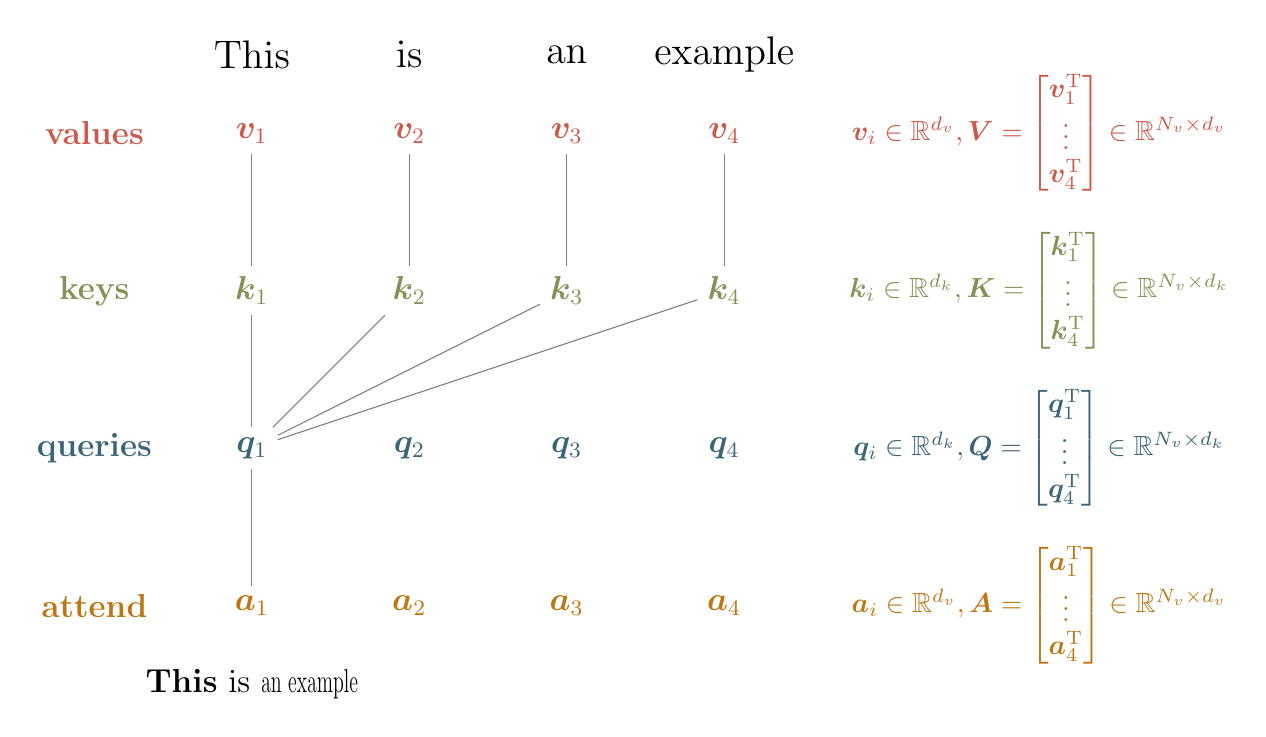
\begin{tikzpicture}[>=latex',thick]

      
      \pgfmathsetmacro{\textY}{2}
      \pgfmathsetmacro{\valuesY}{1}
      \pgfmathsetmacro{\keysY}{-1}
      \pgfmathsetmacro{\queriesY}{-3}
      \pgfmathsetmacro{\attendY}{-5}
      \pgfmathsetmacro{\newTextY}{-6}

      % TEXT
      \node [name=t1] at (0,\textY) {\Large{This}};
      \node [name=t2] at (2,\textY) {\Large{is}};
      \node [name=t3] at (4,\textY) {\Large{an}};
      \node [name=t4] at (6,\textY) {\Large{example}};

      % New Text
      \node [name=tn1] at (0,\newTextY) {\large{\textbf{This} is \scalebox{0.6}[1]{an example}}};

      % attended
      \node  at (-2,\attendY) {\large{\textbf{\textcolor{myorange}{attend}}}};
      \node [name=a1] at (0, \attendY) {\large{\textcolor{myorange}{$\boldsymbol{a}_1$}}};
      \node [name=a2] at (2, \attendY) {\large{\textcolor{myorange}{$\boldsymbol{a}_2$}}};
      \node [name=a3] at (4, \attendY) {\large{\textcolor{myorange}{$\boldsymbol{a}_3$}}};
      \node [name=a4] at (6, \attendY) {\large{\textcolor{myorange}{$\boldsymbol{a}_4$}}};
      \node at (10, \attendY)
      {\textcolor{myorange}{$
          \boldsymbol{a}_i \in \mathbb{R}^{d_v}, 
          \boldsymbol{A} = \begin{bmatrix}
            \boldsymbol{a}_1^{\text{T}} \\ \vdots \\
            \boldsymbol{a}_4^{\text{T}} \end{bmatrix} \in \mathbb{R}^{N_v \times
            d_v}$}}; 



      % values
      \node  at (-2,\valuesY) {\large{\textbf{\textcolor{myred}{values}}}};
      \node [name=v1] at (0, \valuesY) {\large{\textcolor{myred}{$\boldsymbol{v}_1$}}};
      \node [name=v2] at (2, \valuesY) {\large{\textcolor{myred}{$\boldsymbol{v}_2$}}};
      \node [name=v3] at (4, \valuesY) {\large{\textcolor{myred}{$\boldsymbol{v}_3$}}};
      \node [name=v4] at (6, \valuesY) {\large{\textcolor{myred}{$\boldsymbol{v}_4$}}};

      \node at (10, \valuesY)
      {\textcolor{myred}{$
          \boldsymbol{v}_i \in \mathbb{R}^{d_v}, 
          \boldsymbol{V} = \begin{bmatrix}
            \boldsymbol{v}_1^{\text{T}} \\ \vdots \\
            \boldsymbol{v}_4^{\text{T}} \end{bmatrix} \in \mathbb{R}^{N_v \times
            d_v}$}}; 

      % keys 
      \node  at (-2,\keysY) {\large{\textbf{\textcolor{mygreen}{keys}}}};
      \node [name=k1] at (0, \keysY) {\large{\textcolor{mygreen}{$\boldsymbol{k}_1$}}};
      \node [name=k2] at (2, \keysY) {\large{\textcolor{mygreen}{$\boldsymbol{k}_2$}}};
      \node [name=k3] at (4, \keysY) {\large{\textcolor{mygreen}{$\boldsymbol{k}_3$}}};
      \node [name=k4] at (6, \keysY) {\large{\textcolor{mygreen}{$\boldsymbol{k}_4$}}};


      \node at (10, \keysY)
      {\textcolor{mygreen}{$
          \boldsymbol{k}_i \in \mathbb{R}^{d_k}, 
          \boldsymbol{K} = \begin{bmatrix}
            \boldsymbol{k}_1^{\text{T}} \\ \vdots \\
            \boldsymbol{k}_4^{\text{T}} \end{bmatrix} \in \mathbb{R}^{N_v \times
            d_k}$}}; 

      % queries
      \node at (-2,\queriesY) {\large{\textbf{\textcolor{myblue}{queries}}}};
      \node [name=q1] at (0, \queriesY) {\large{\textcolor{myblue}{$\boldsymbol{q}_1$}}};
      \node [name=q2] at (2, \queriesY) {\large{\textcolor{myblue}{$\boldsymbol{q}_2$}}};
      \node [name=q3] at (4, \queriesY) {\large{\textcolor{myblue}{$\boldsymbol{q}_3$}}};
      \node [name=q4] at (6, \queriesY) {\large{\textcolor{myblue}{$\boldsymbol{q}_4$}}};

      \draw [-, thin, color=gray] (a1) -- (q1);

      \draw [-, thin, color=gray] (q1) -- (k1);
      \draw [-, thin, color=gray] (q1) -- (k2);
      \draw [-, thin, color=gray] (q1) -- (k3);
      \draw [-, thin, color=gray] (q1) -- (k4);

      \draw [-, thin, color=gray] (k1) -- (v1);
      \draw [-, thin, color=gray] (k2) -- (v2);
      \draw [-, thin, color=gray] (k3) -- (v3);
      \draw [-, thin, color=gray] (k4) -- (v4);

    \node at (10, \queriesY)
      {\textcolor{myblue}{$
          \boldsymbol{q}_i \in \mathbb{R}^{d_k}, 
          \boldsymbol{Q} = \begin{bmatrix}
            \boldsymbol{q}_1^{\text{T}} \\ \vdots \\
            \boldsymbol{q}_4^{\text{T}} \end{bmatrix} \in \mathbb{R}^{N_v \times
            d_k}$}}; 




    \end{tikzpicture}
\end{document}
